\documentclass[10pt]{beamer}

\setbeamertemplate{note page}[default]
%\setbeameroption{hide notes}
\setbeameroption{show notes}


\usetheme[progressbar=frametitle]{metropolis}
\usepackage{appendixnumberbeamer}

\usepackage{booktabs}
\usepackage[scale=2]{ccicons}

\usepackage{pgfplots}
\usepgfplotslibrary{dateplot}
\usepackage{multicol}
\setlength{\columnsep}{1.5cm}

\usepackage{animate}
\usepackage{lmodern}
\usepackage[T1]{fontenc}
\usepackage{mathtools}
\usepackage{graphicx}
\usepackage{caption}
\usepackage[export]{adjustbox}

\definecolor{set1}{RGB}{228, 26, 28}
\definecolor{set2}{RGB}{77, 175, 74}
\definecolor{set3}{RGB}{255, 127, 0}
\definecolor{set4}{RGB}{166, 86, 40}
\definecolor{set5}{RGB}{153, 153, 153}

\usepackage{xspace}
\newcommand{\themename}{\textbf{\textsc{metropolis}}\xspace}

\newcommand\Fontvi{\fontsize{8}{9}\selectfont}
\newcommand\Fontvr{\fontsize{6}{7}\selectfont}

\setbeamerfont{parent A}{size=\small}


\title{Dissemination}
\subtitle{Building a Decision Support System}
% \date{\today}
\date{}
\author{Michoel Snow, M.D. Ph.D. and Glen Ferguson, Ph.D.}
\institute{Center for Health Data Innovations}

\begin{document}

\maketitle

\begin{frame}{Bioinformatics Pipeline}
	\begin{center}
		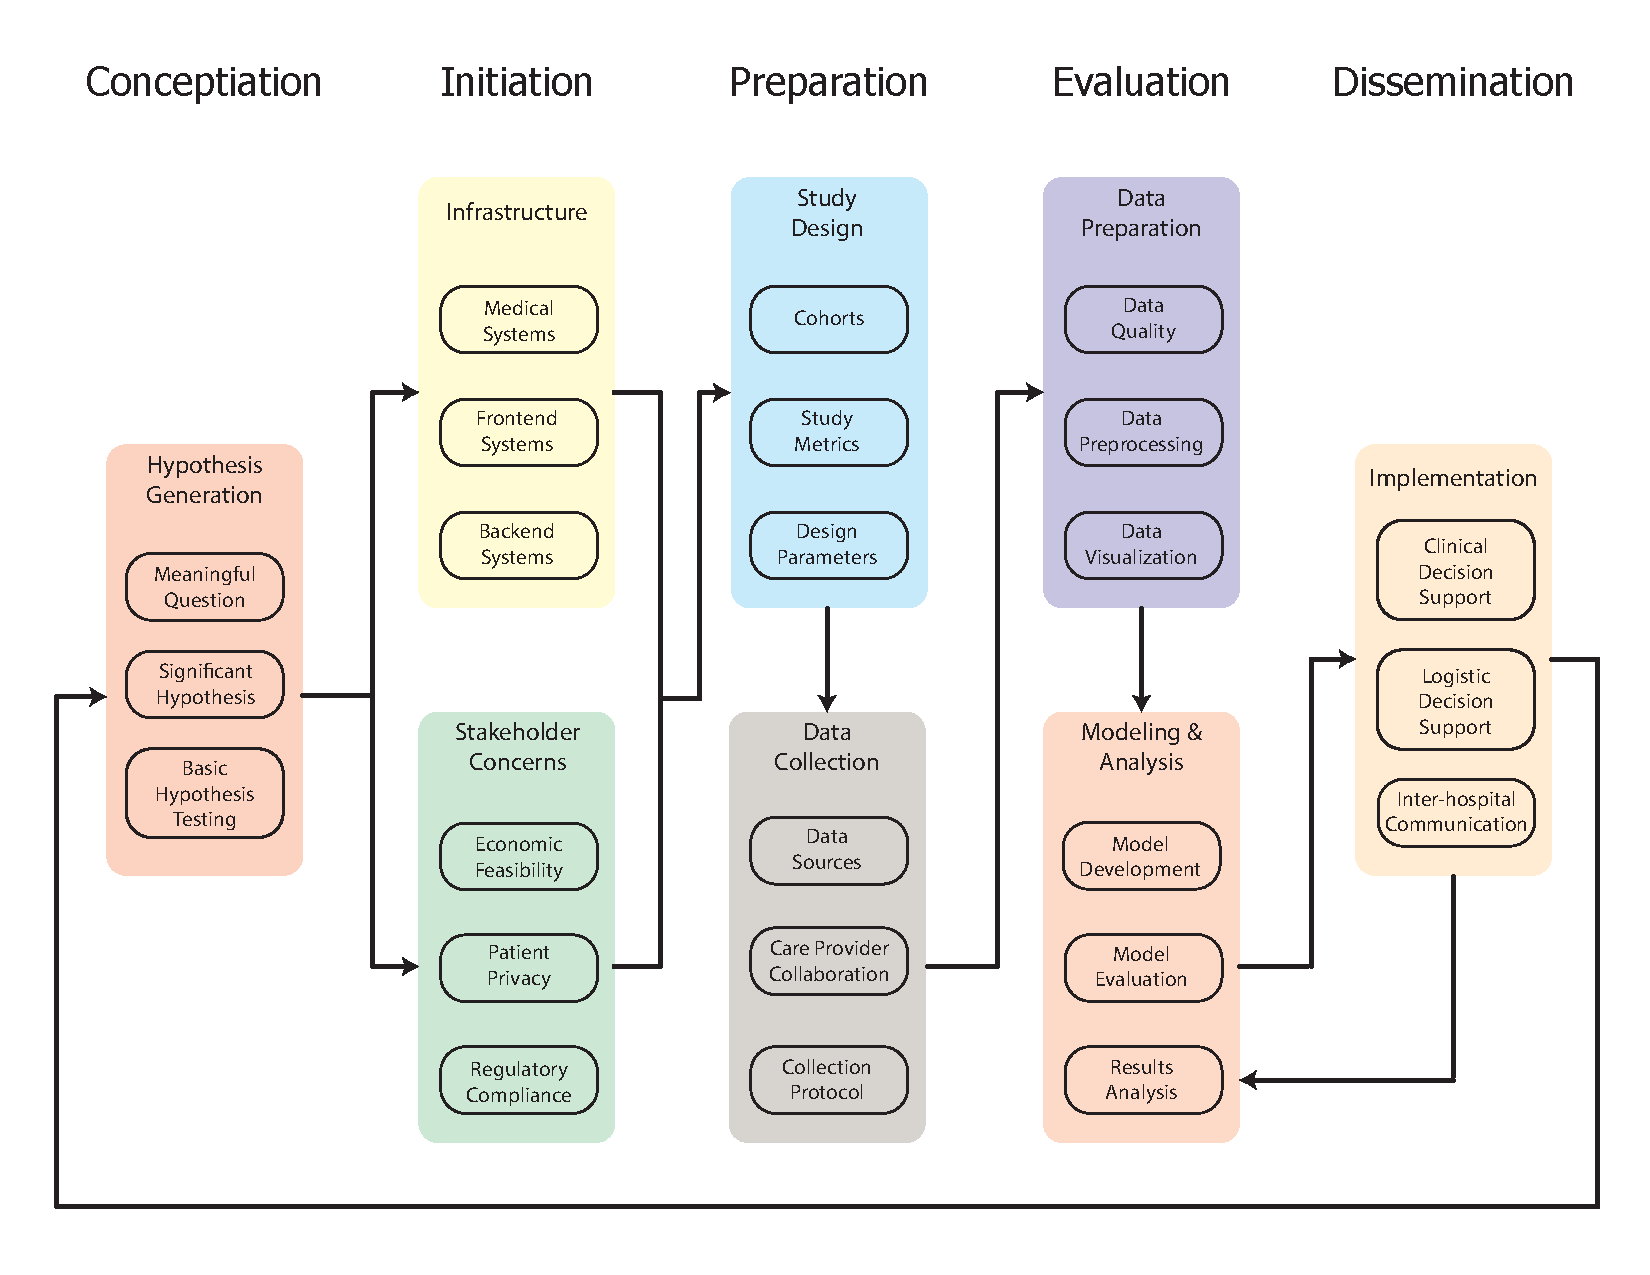
\includegraphics[width=0.8\textwidth]{images/informatics_pipeline.pdf}	
	\end{center}
\end{frame}


\begin{frame}{Dissemination}
	\begin{center}
		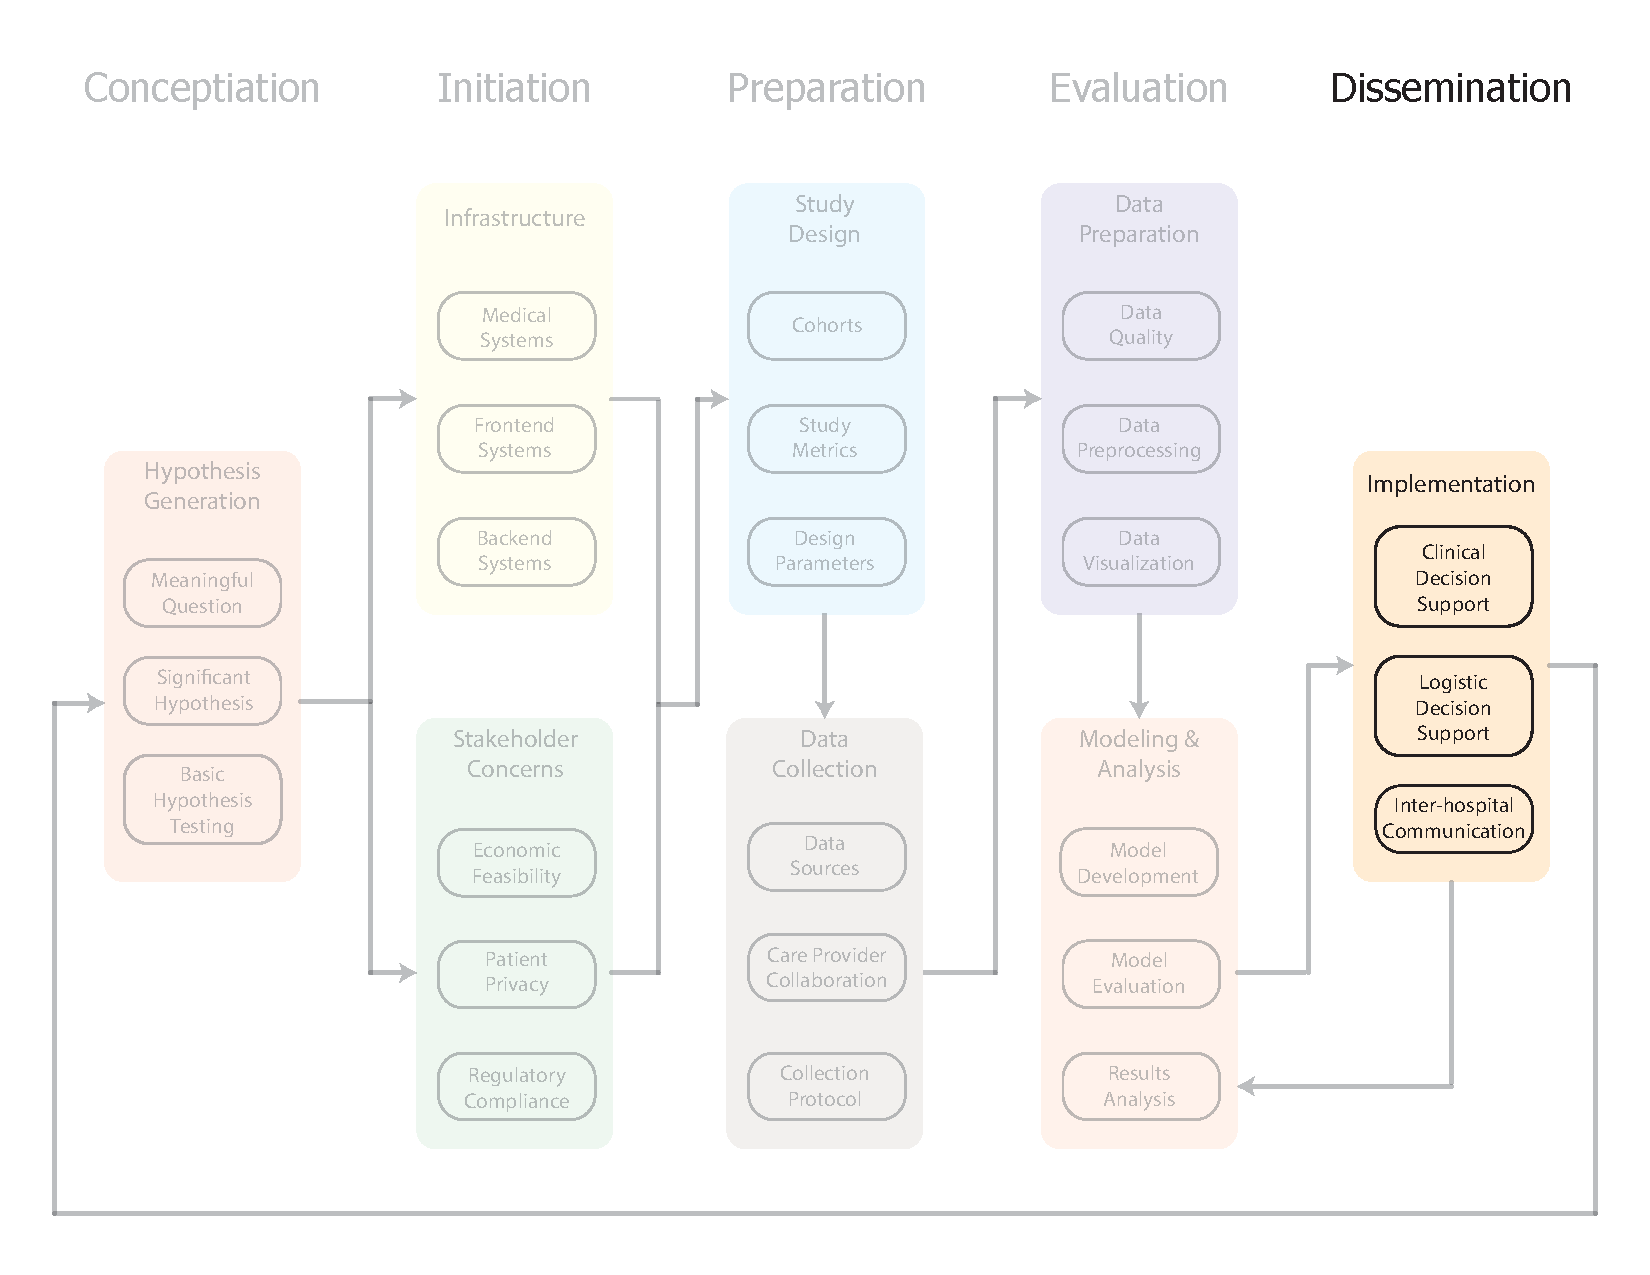
\includegraphics[width=0.8\textwidth]{images/informatics_pipeline_implementation.pdf}
	\end{center}
\end{frame}

\section{Clinical Decision Support Systems}

\begin{frame}{What is Clinical Decision Support?}
Definitions?
\pause
\begin{itemize}
	\item A health information technology designed provide assistance in making medical decisions
	\pause
	\item Linking health observations with health knowledge to influence health choices by providers
	\pause
	\item A process for ensuring that health-related decisions and actions are informed by pertinent information and clinical knowledge to enhance health and health care delivery
\end{itemize}
%	\begin{center}
%		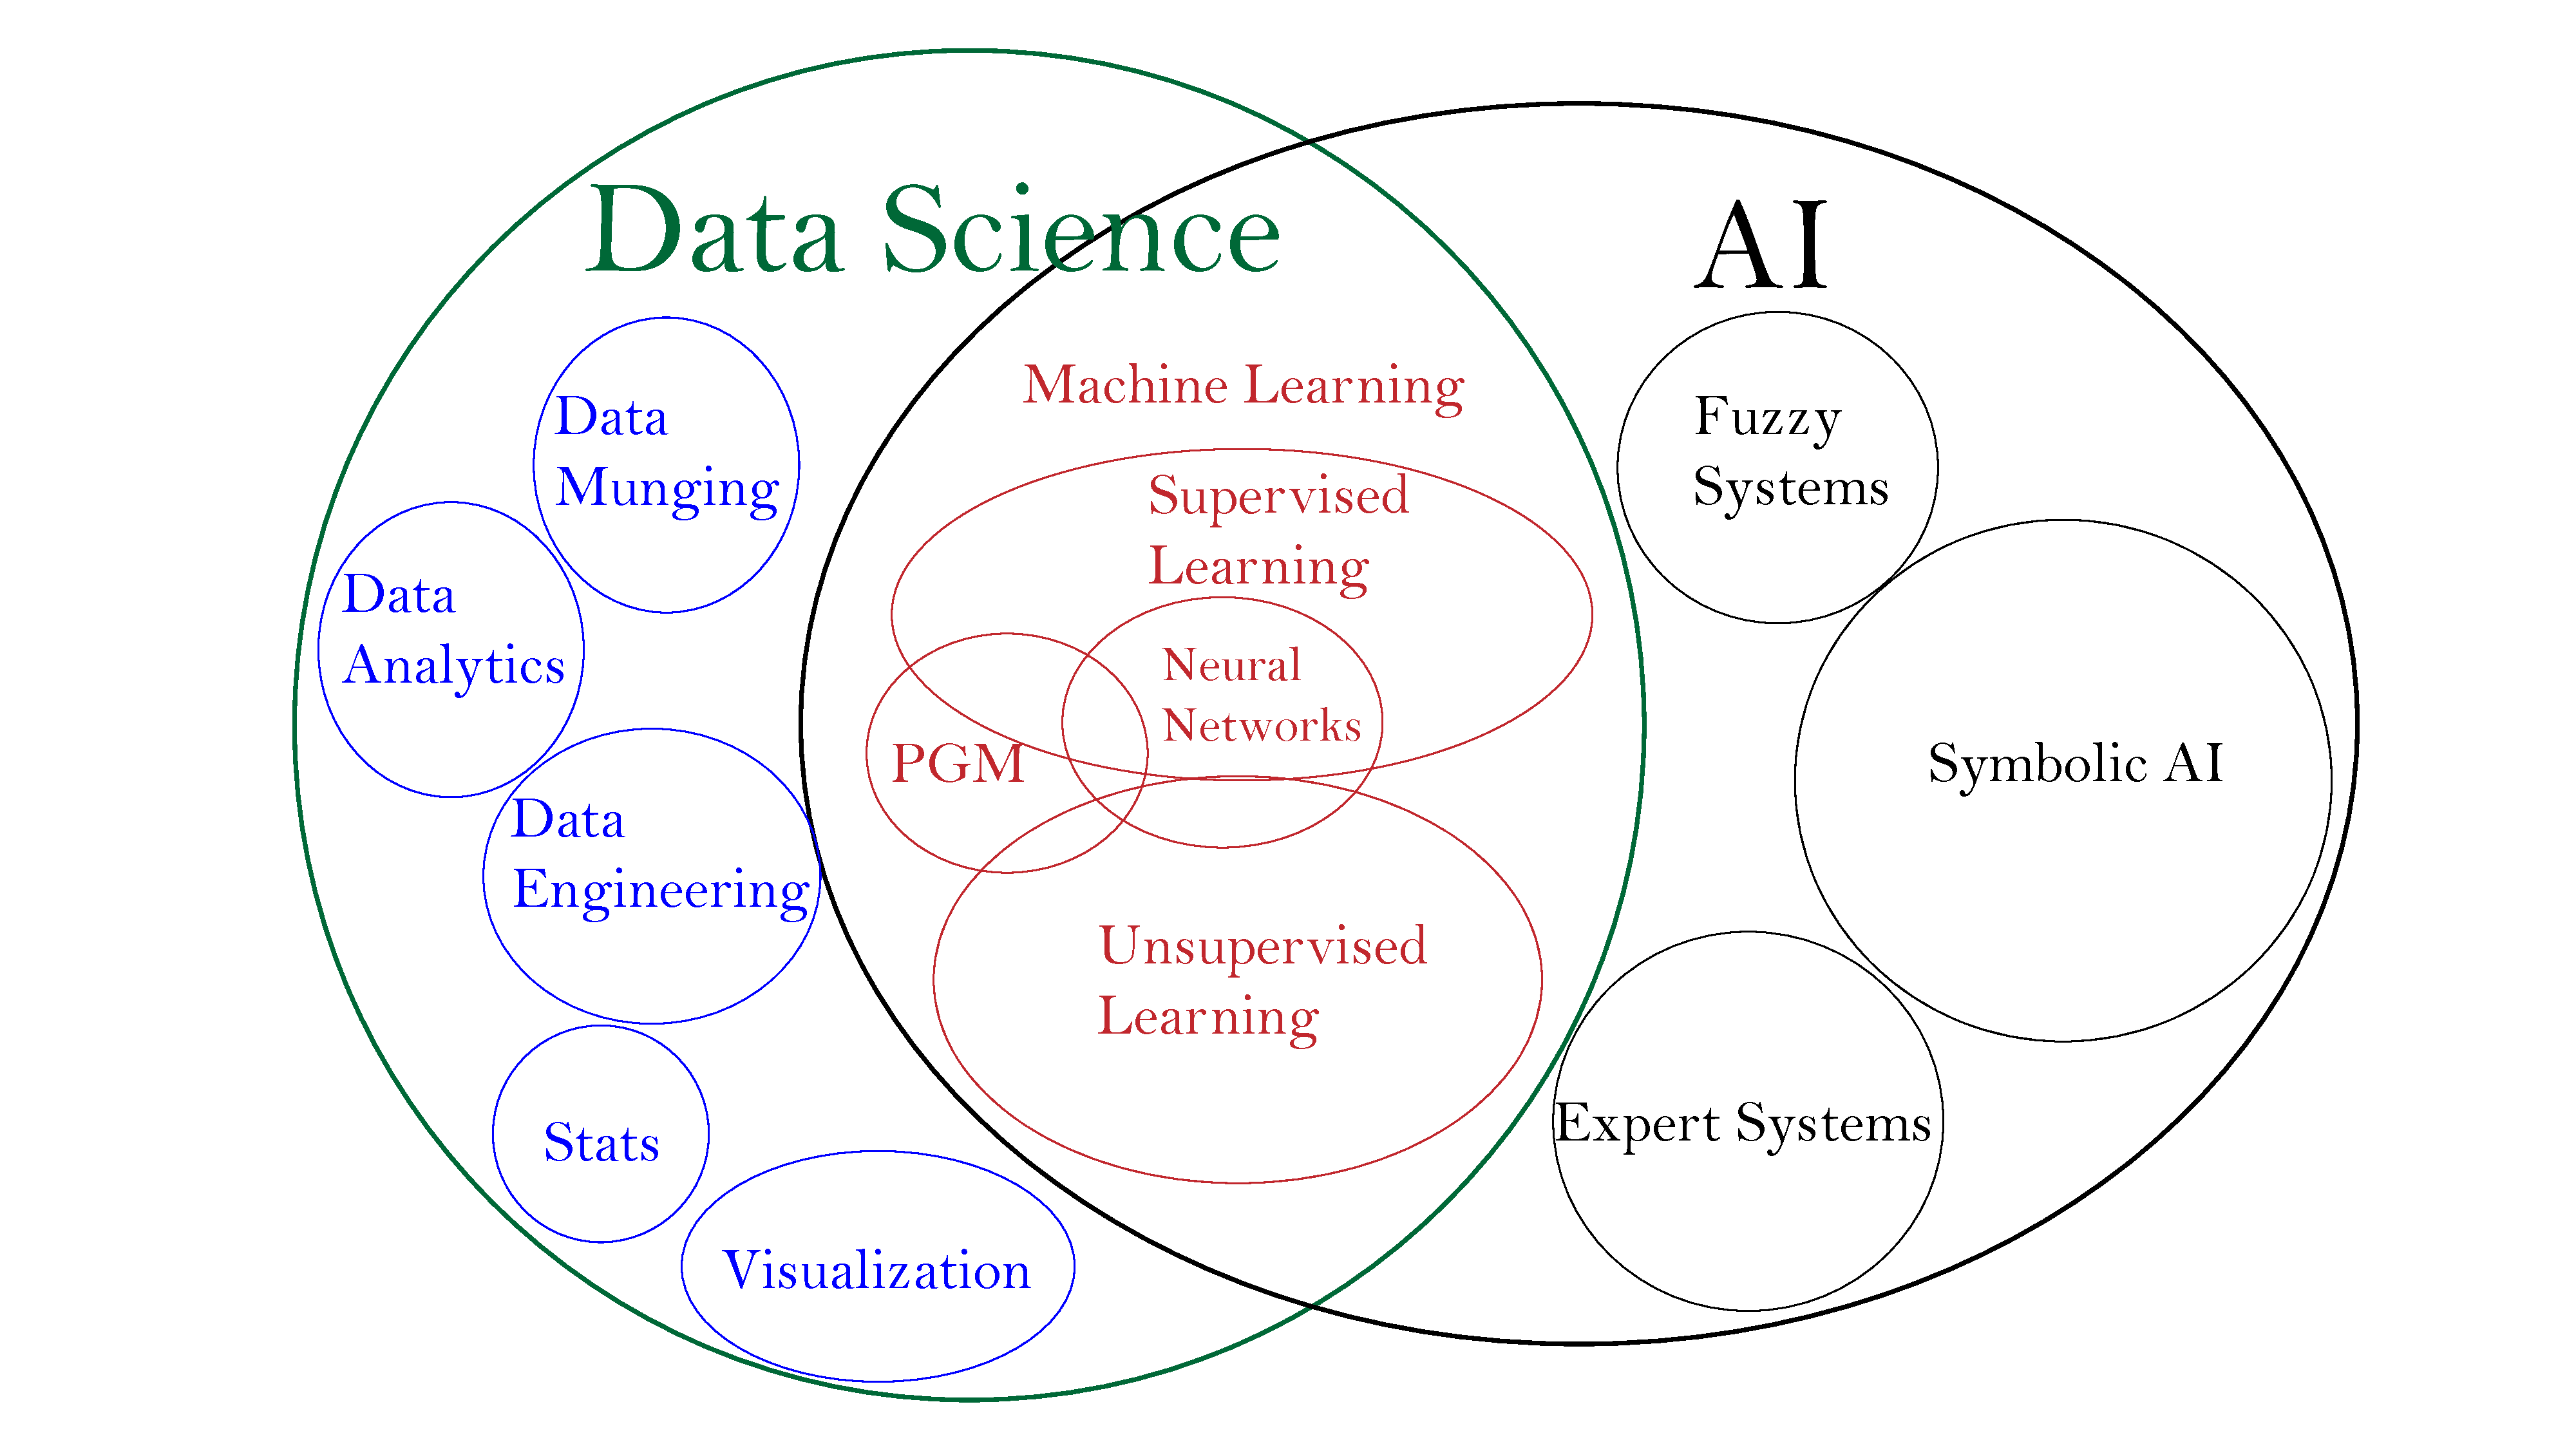
\includegraphics[width=1.2\textwidth, center, trim=-8cm -8cm 0 0cm]{images/overlapping_dis.pdf}
%	\end{center}
\end{frame}

\begin{frame}{Five Rights of CDS Framework?}
What are the important factors to consider when implemented \emph{any} CDS system.
\pause
	\begin{center}
		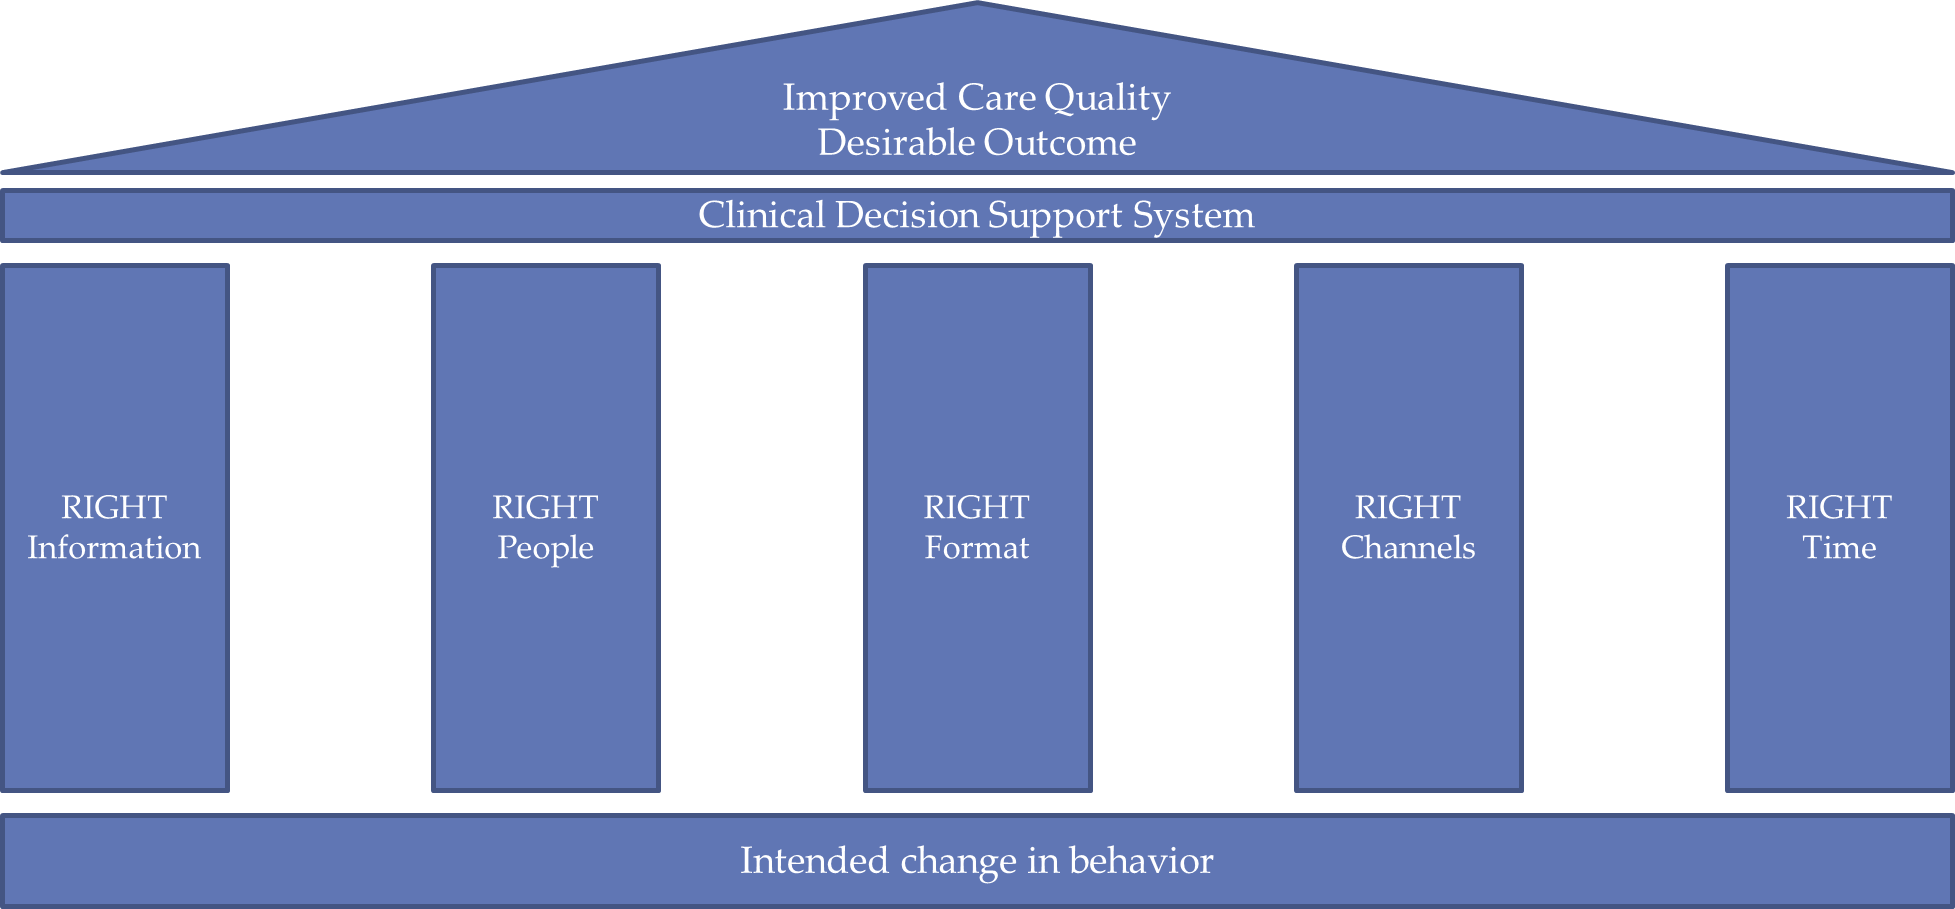
\includegraphics[width=1.0\textwidth, center, trim=0cm 0cm 0 0cm]{images/five_rights.png}
	\end{center}
\end{frame}

\section{Best Practice Advisories}

\begin{frame}{A CDS Example}
Best Practice Alerts (BPAs) are messages to health care providers concerning a patient status or condition.
\pause
\begin{itemize}
	\item Delivered through an EMR
	\pause
	\item Built based on clinical intent
	\pause
	\item Often require a response from the provider
	\pause
	\item Contain criteria for trigger actions and filters for display
\end{itemize}
\end{frame}

\begin{frame}{Understanding how BPAs Currently Work}
Current BPA Framework
	\begin{center}
		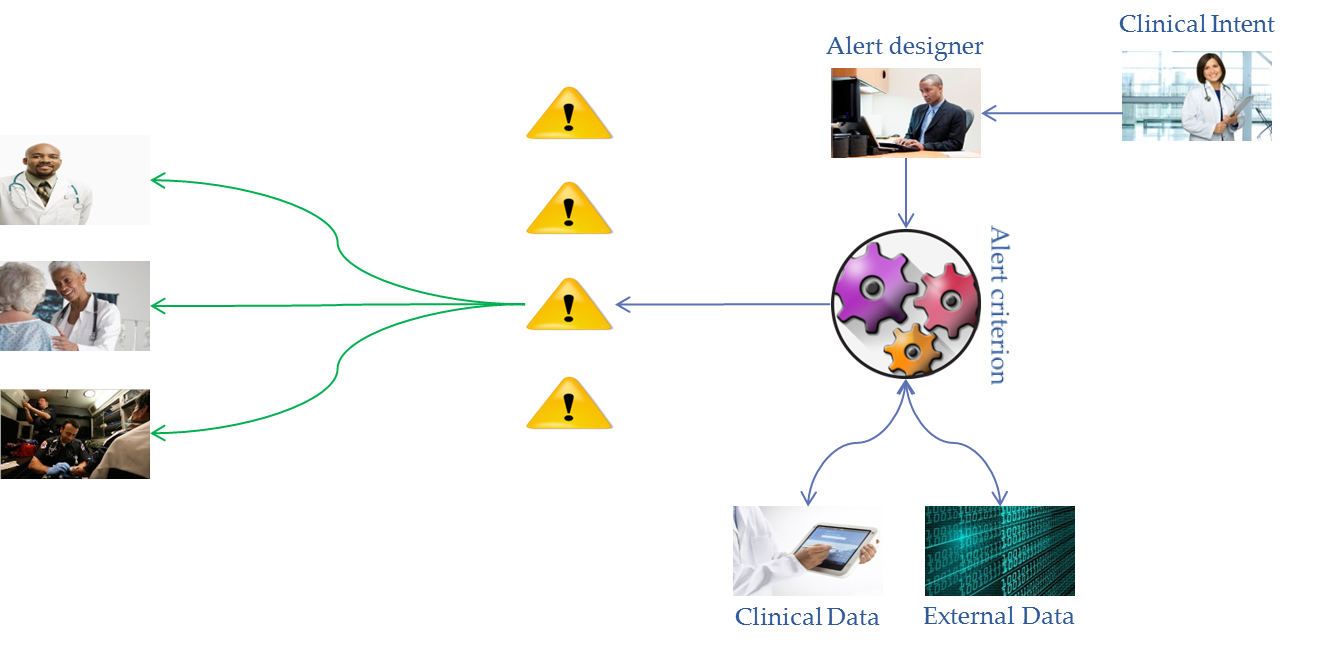
\includegraphics[width=1.2\textwidth, center, trim=-1cm -1cm -1cm -1cm]{images/current_framework.png}
	\end{center}
\end{frame}

\begin{frame}{Understanding how BPAs Currently Work}
Current BPA Framework
	\begin{center}
		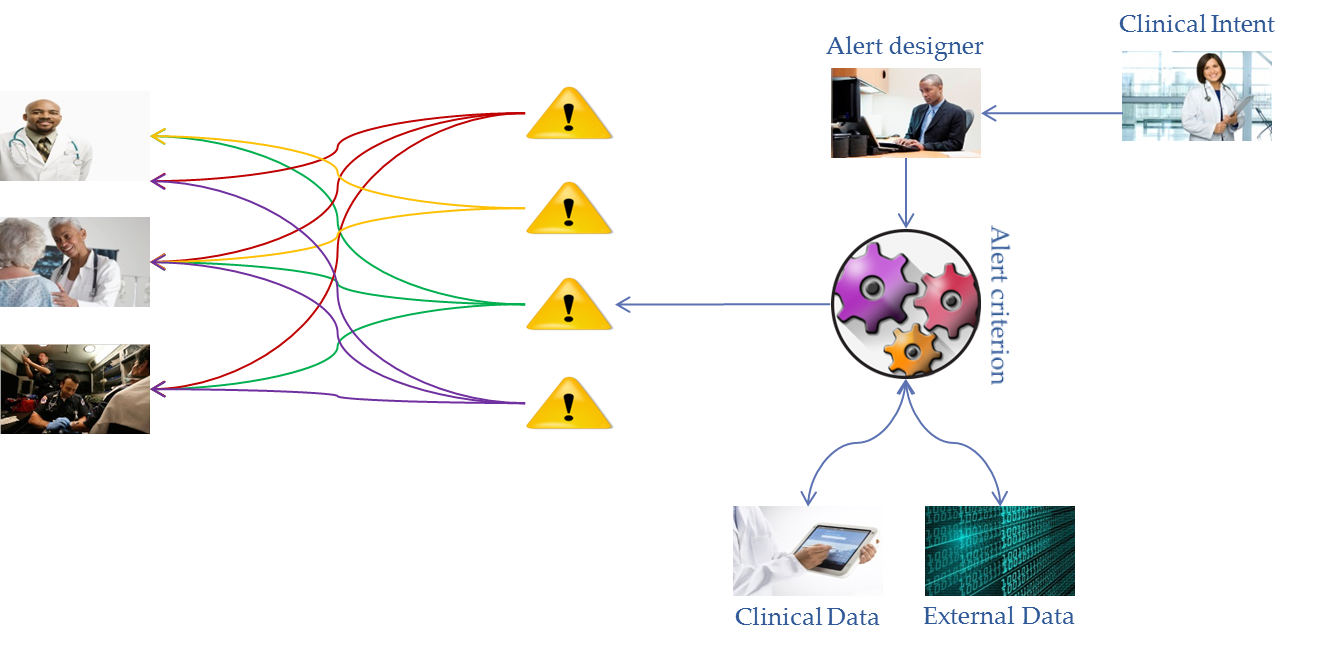
\includegraphics[width=1.2\textwidth, center, trim=-1cm -1cm -1cm -1cm]{images/current_framework_2.png}
	\end{center}
\end{frame}

\begin{frame}{Understanding how BPAs Currently Work}
Problems with the current framework
\pause
\begin{itemize}
	\item Right information?
	\pause
	\item Right people?
	\pause
	\item Right format?
	\pause
	\item Right channels?
	\pause
	\item Right time?
\end{itemize}
\end{frame}

\begin{frame}{Anatomy of a BPA}
	\begin{center}
		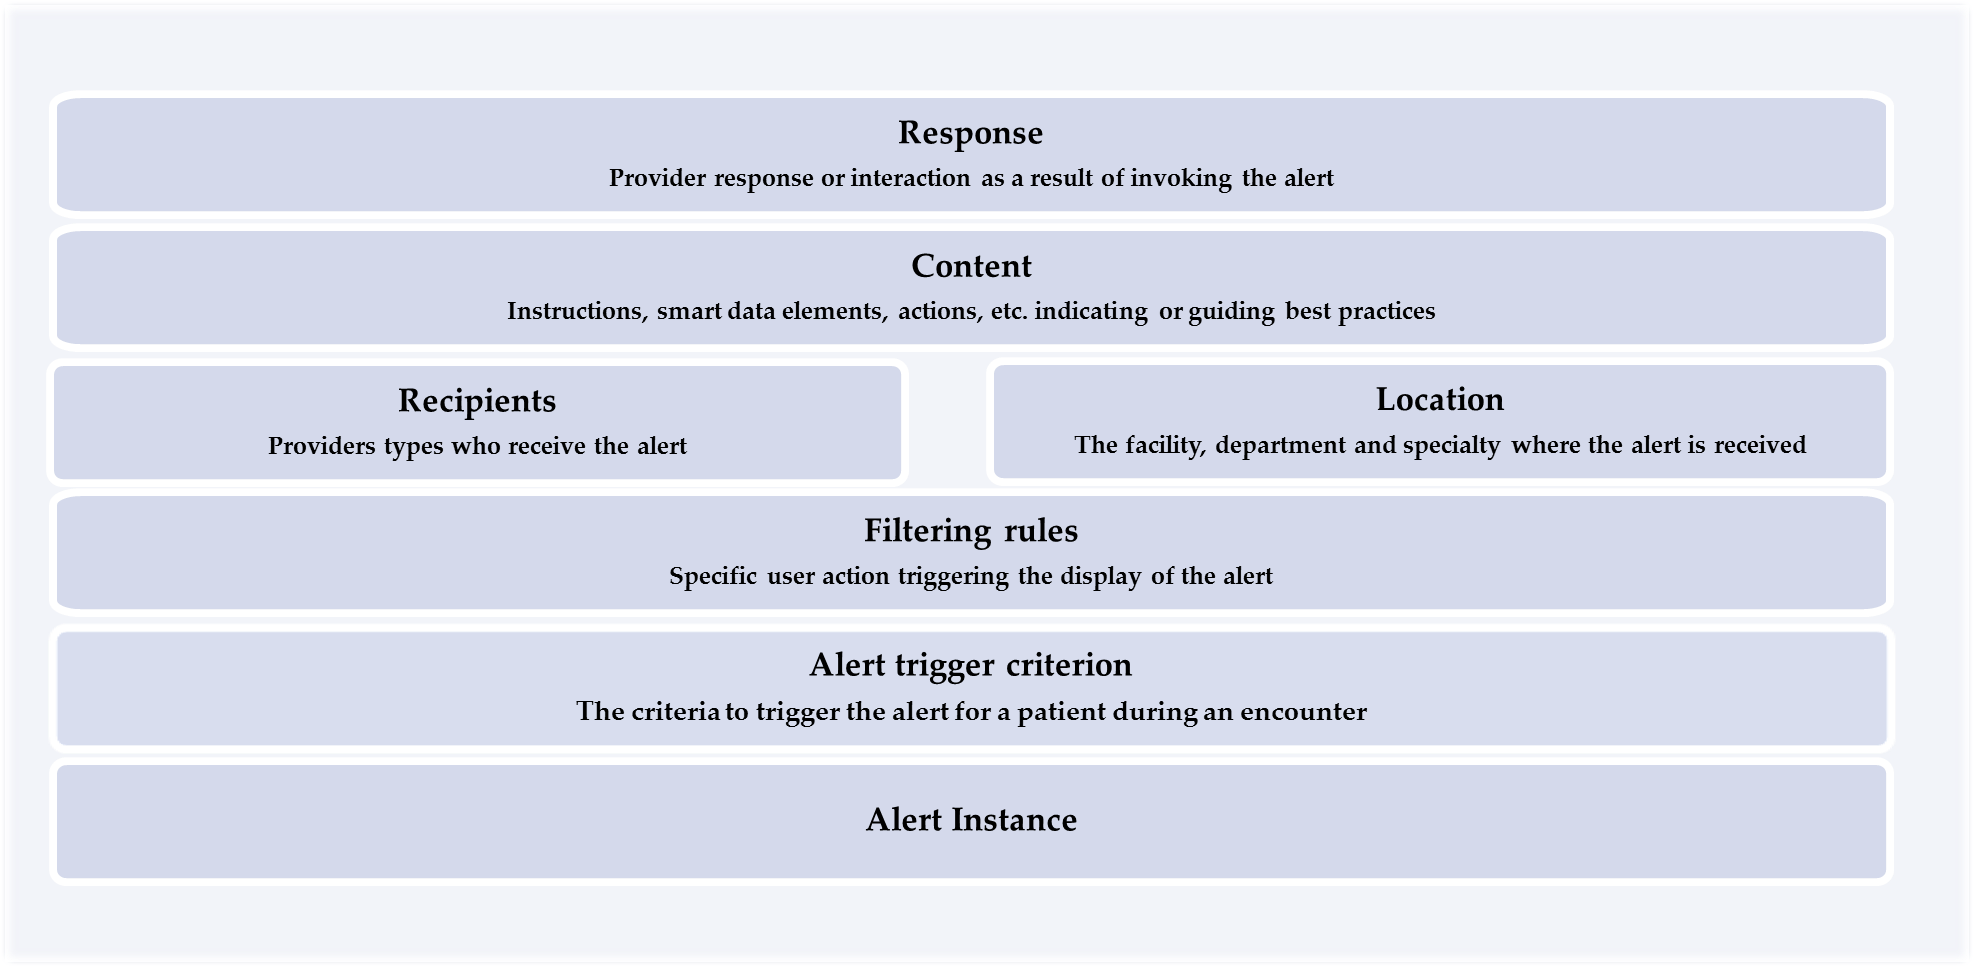
\includegraphics[width=1.2\textwidth, center, trim=-1cm -1cm -1cm -1cm]{images/alert_anatomy.png}
	\end{center}
\end{frame}

\begin{frame}{BPA Life-cycle}
	\begin{center}
		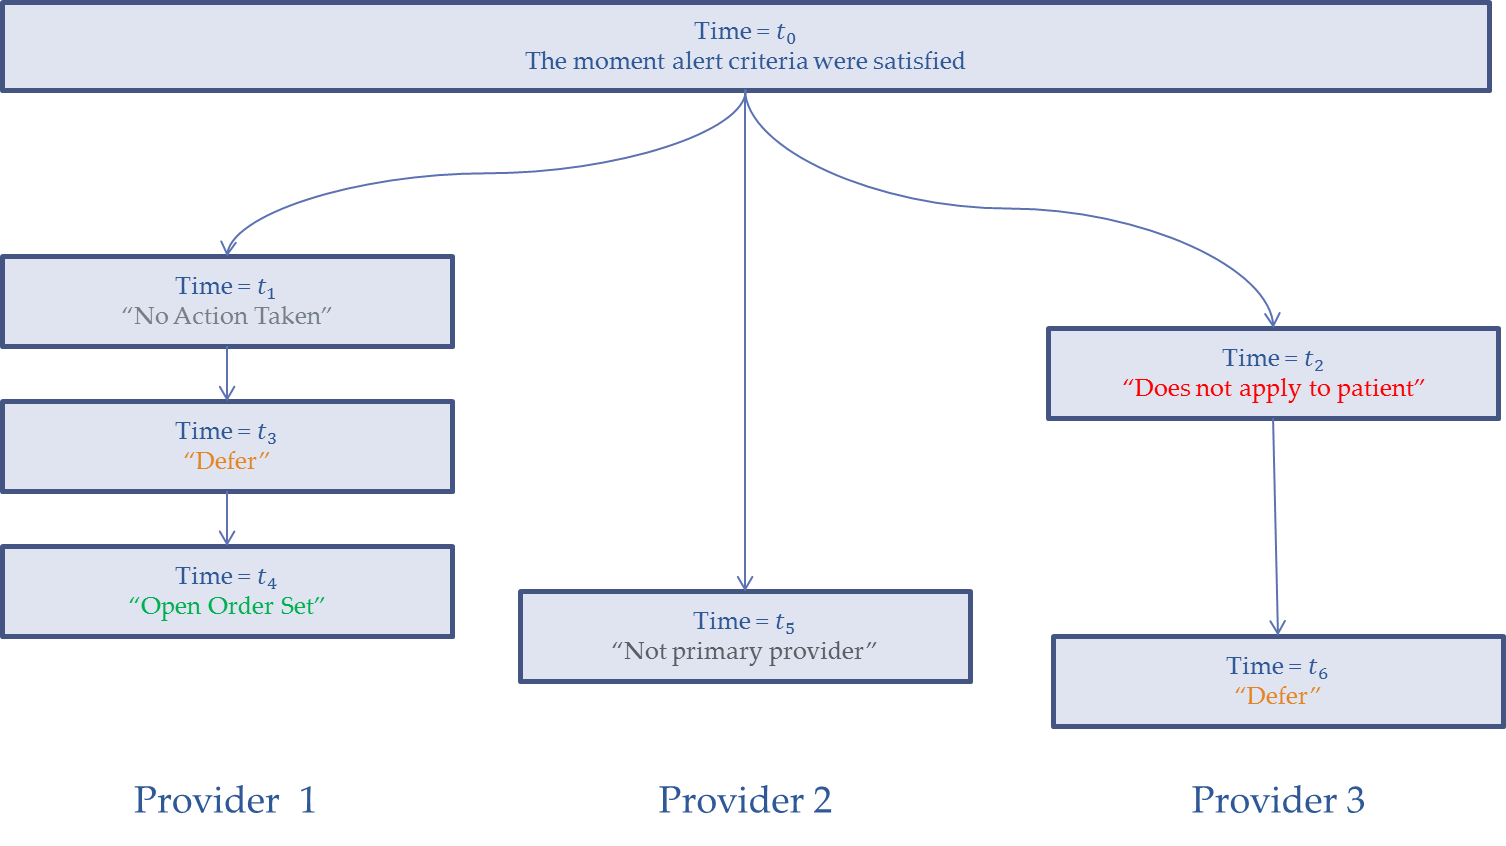
\includegraphics[width=1.2\textwidth, center, trim=-1cm -1cm -1cm -1cm]{images/BPA_lifecycle.png}
	\end{center}
\end{frame}

\begin{frame}{BPA Life-cycle}
	\begin{center}
		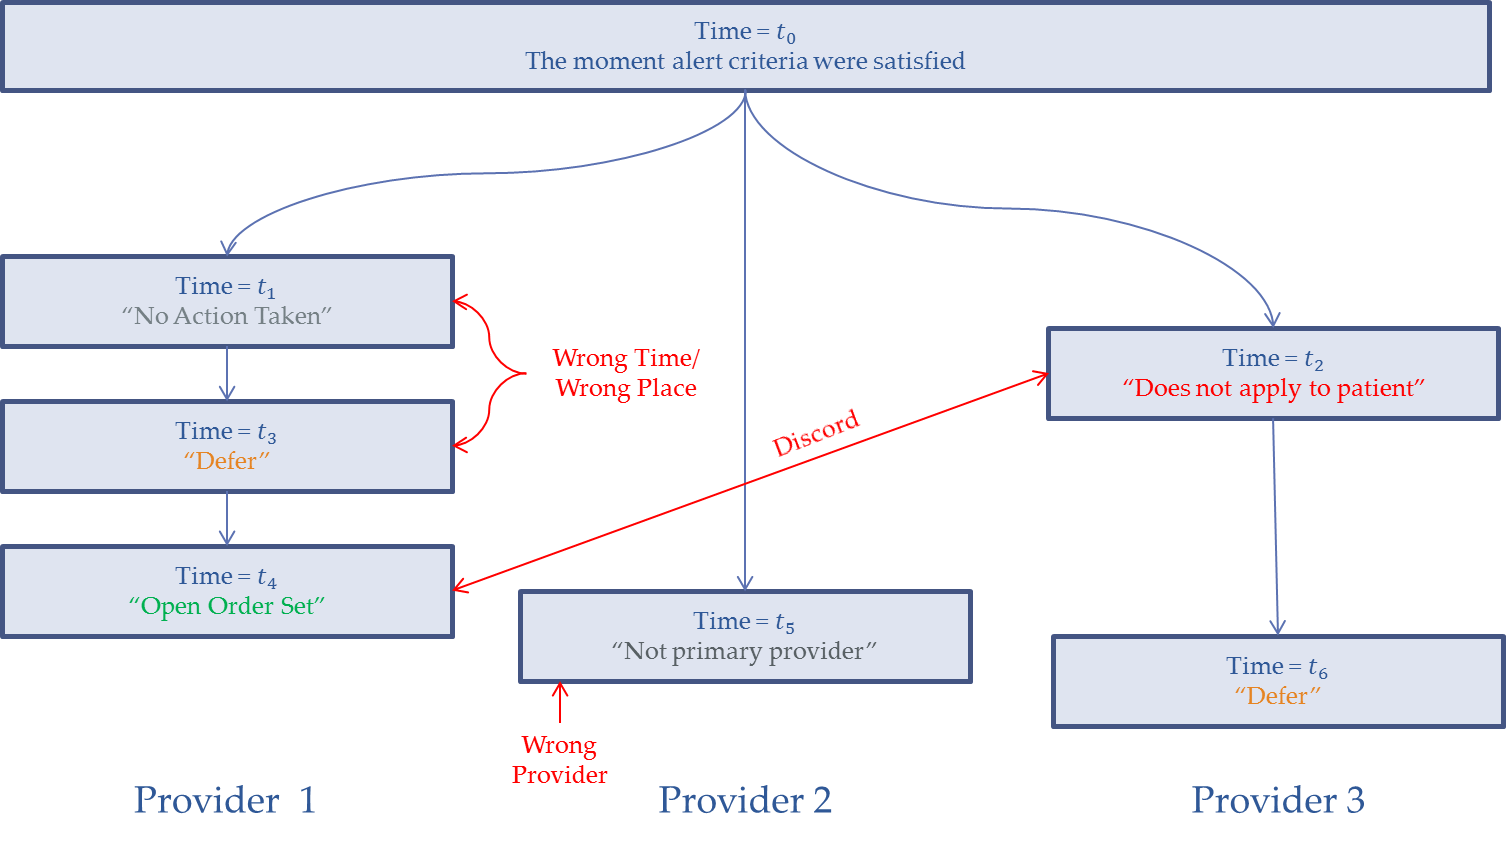
\includegraphics[width=1.2\textwidth, center, trim=-1cm -1cm -1cm -1cm]{images/BPA_lifecycle_2.png}
	\end{center}
\end{frame}

\section{Evaluating Best Practice Advisories}

\begin{frame}{Average BPA Interactions per Provider}
	\begin{center}
		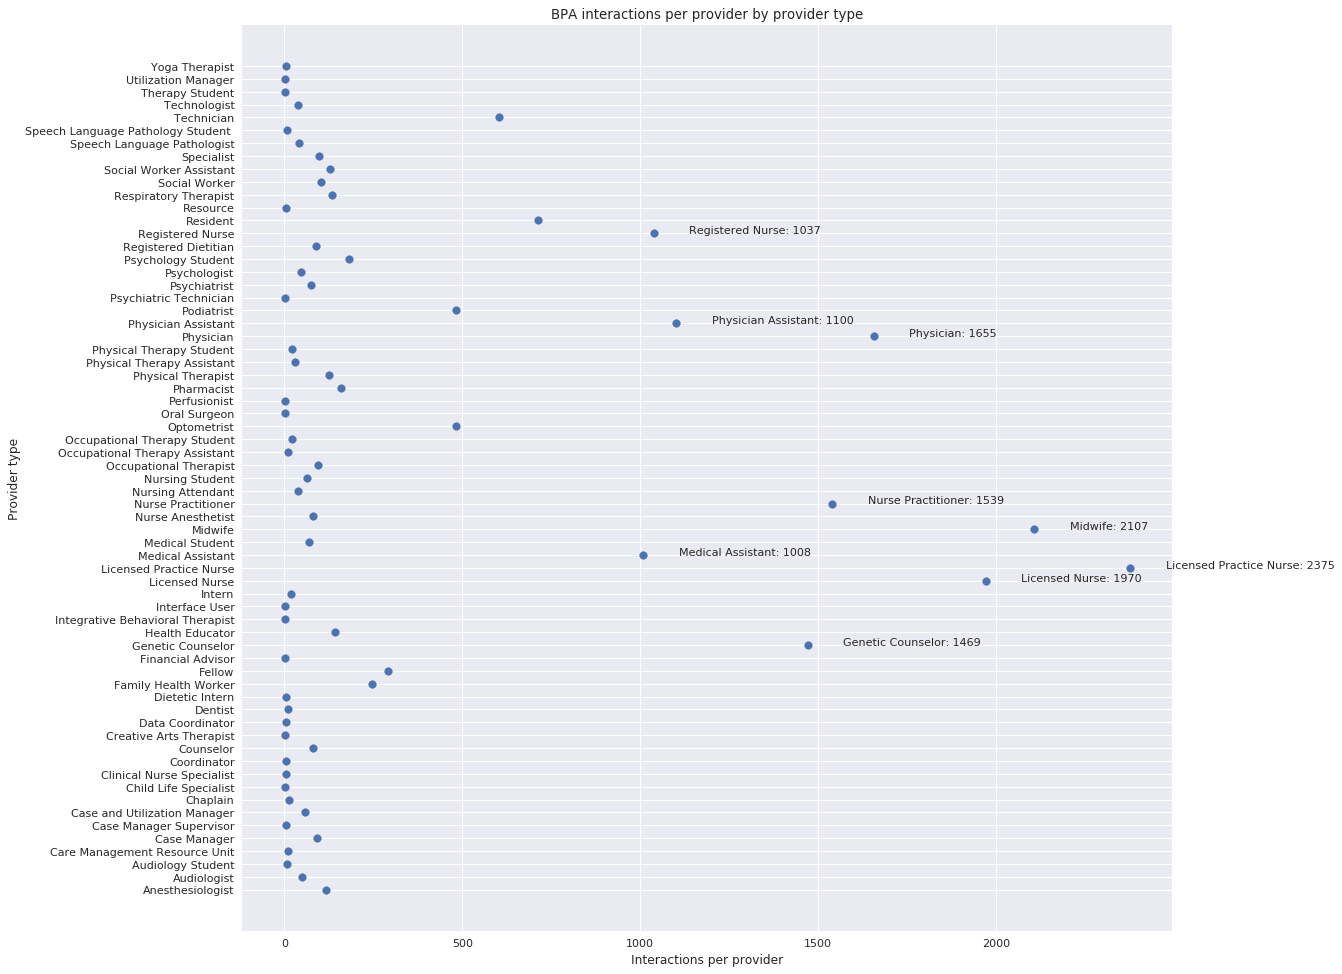
\includegraphics[width=0.9\textwidth, center, trim=0cm 0cm 0cm 0cm]{images/avg_int_per_provider.png}
	\end{center}
\end{frame}

\begin{frame}{BPA types per Provider}
	\begin{center}
		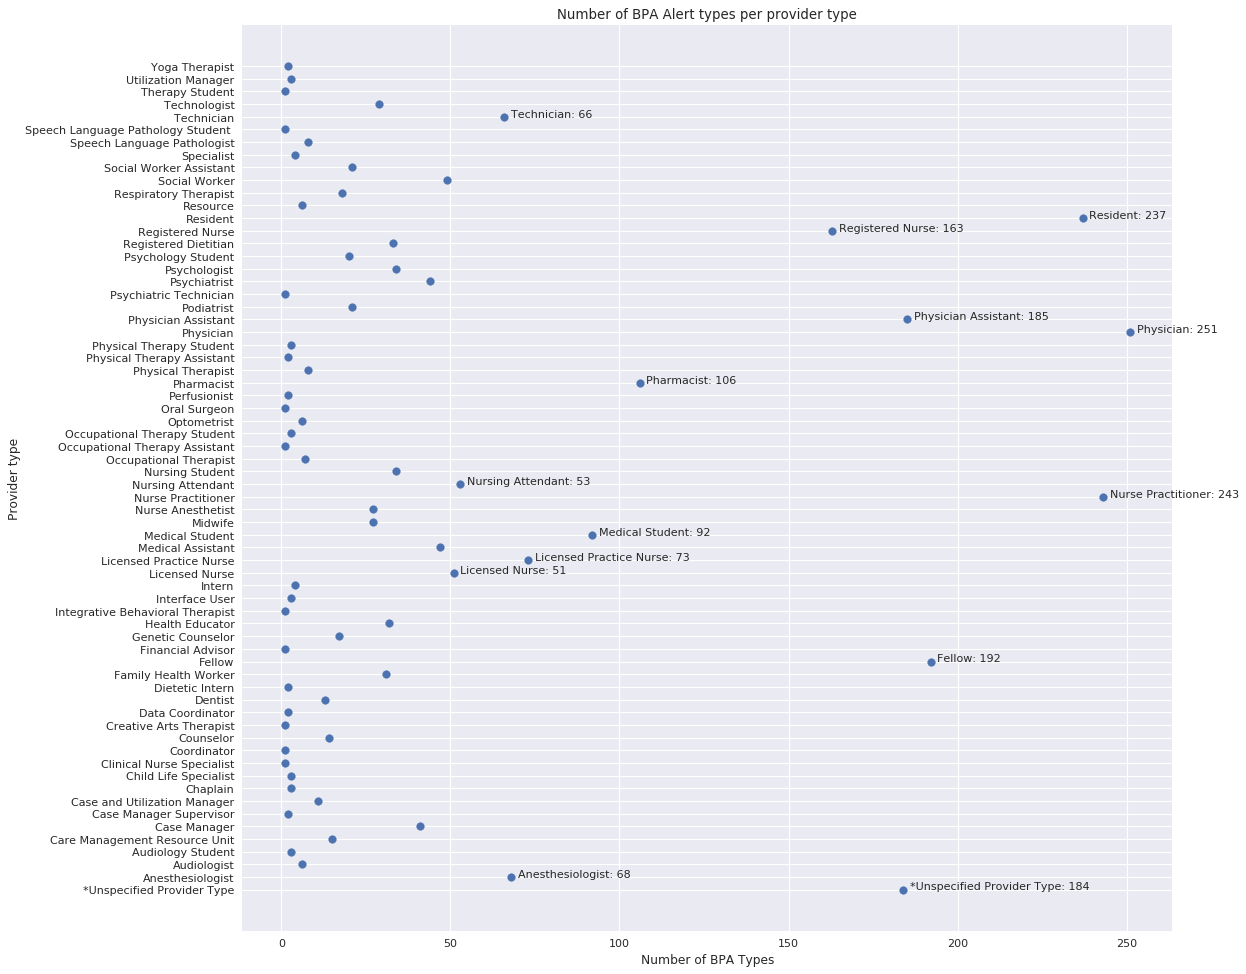
\includegraphics[width=0.9\textwidth, center, trim=0cm 0cm 0cm 0cm]{images/type_per_provider.png}
	\end{center}
\end{frame}

\begin{frame}{Responses to BPAs}
	\begin{center}
		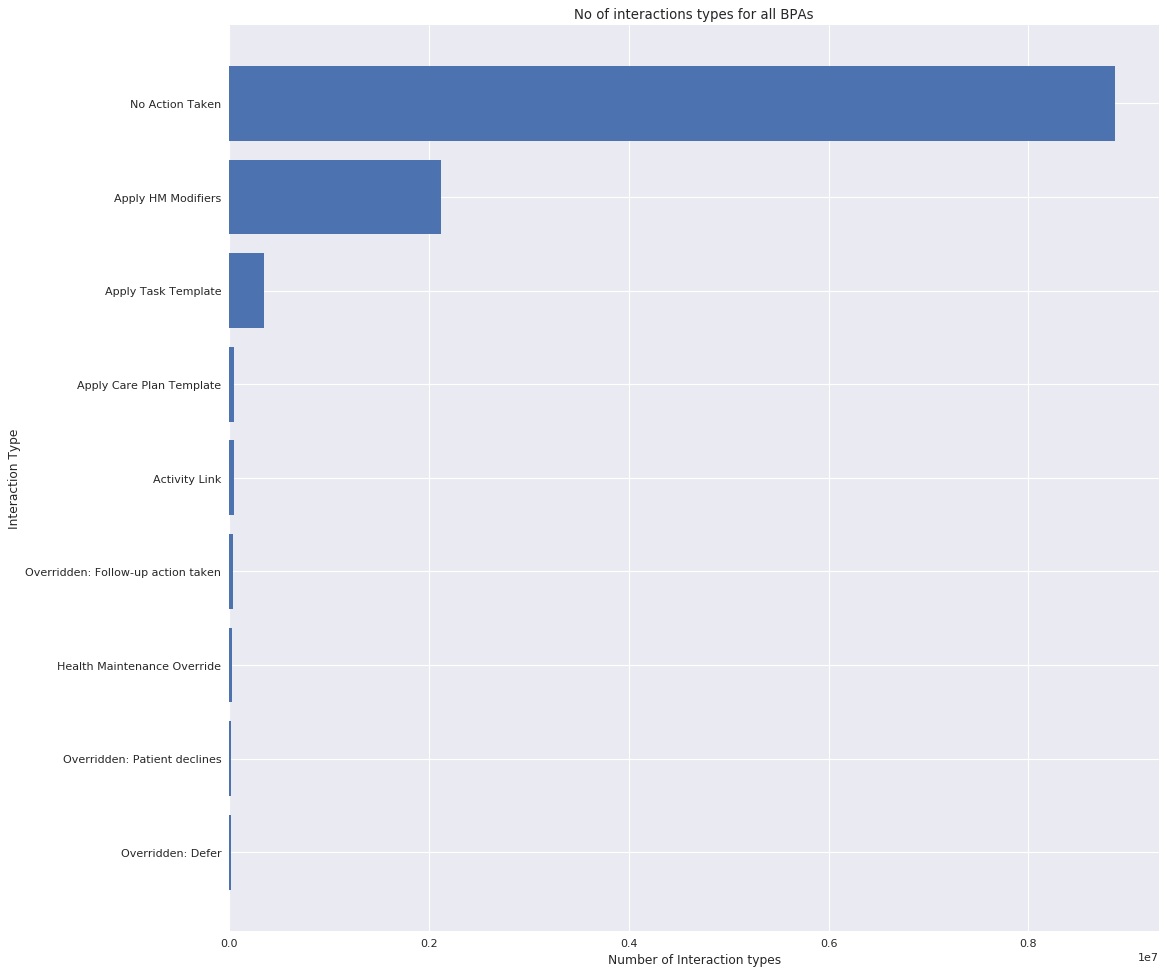
\includegraphics[width=0.9\textwidth, center, trim=0cm 0cm 0cm 0cm]{images/interaction_counts.png}
	\end{center}
\end{frame}

\begin{frame}{Responses to BPAs}
	\begin{center}
		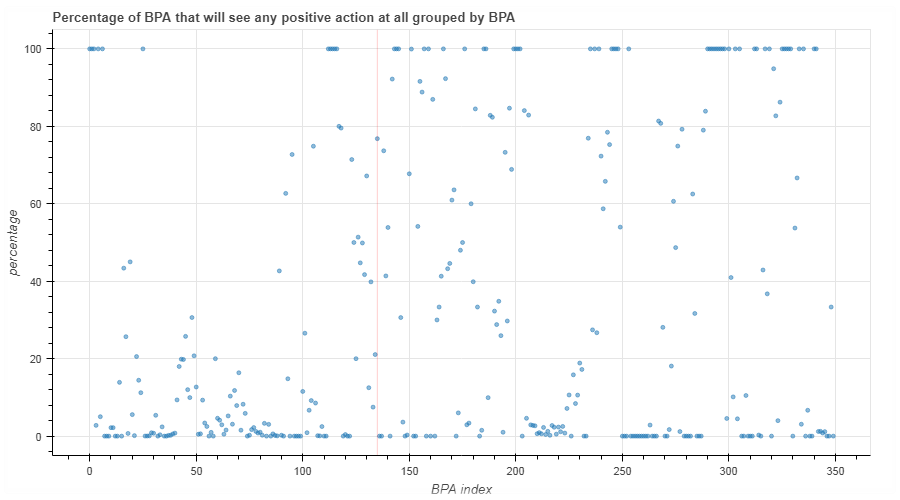
\includegraphics[width=1.1\textwidth, center, trim=0cm 0cm 0cm 0cm]{images/percent_positive_int.png}
	\end{center}
\end{frame}

\begin{frame}{Responses to BPAs}
	\begin{center}
		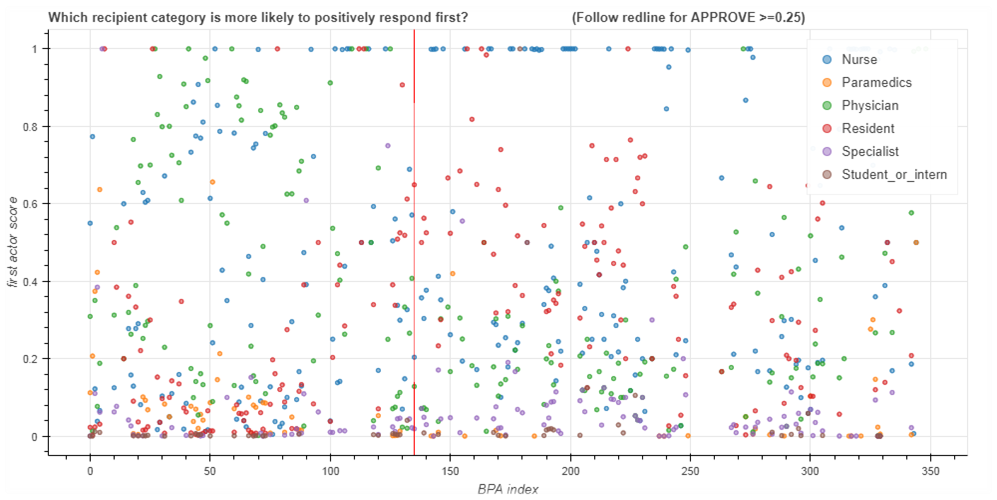
\includegraphics[width=1.1\textwidth, center, trim=0cm 0cm 0cm 0cm]{images/Percentage_first_interaction.png}
	\end{center}
\end{frame}

\begin{frame}{Responses to BPAs}
	\begin{center}
		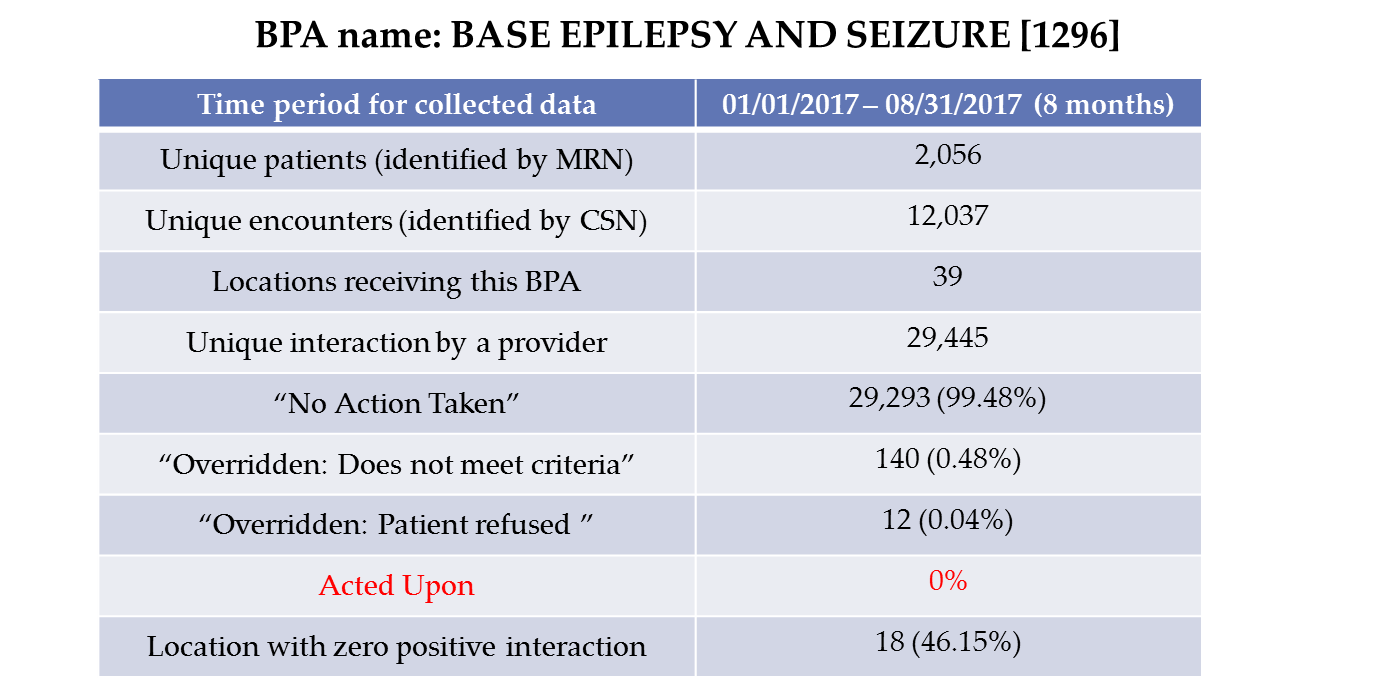
\includegraphics[width=1.0\textwidth, center, trim=0cm 0cm 0cm 0cm]{images/failed_BPA.png}
	\end{center}
\end{frame}

\section{Improving Best Practice Advisories}

\begin{frame}{Building a better BPAs}
Solutions to problems in the current framework
\pause
\begin{itemize}
	\item Right information?
	\item Right people?
	\item Right format?
	\item Right channels?
	\item Right time?
\end{itemize}
\end{frame}

\begin{frame}{Building a better BPAs}
Right information
\begin{itemize}
	\item Method
	\item Testing
	\item Data needs
	\item System maintenance 
\end{itemize}
\end{frame}

\begin{frame}{Building a better BPAs}
Right People
\begin{itemize}
	\item Method
	\item Testing
	\item Data needs
	\item System maintenance 
\end{itemize}
\end{frame}

\begin{frame}{Building a better BPAs}
Right People
\begin{itemize}
	\item Method
	\item Testing
	\item Data needs
	\item System maintenance 
\end{itemize}
\end{frame}

\begin{frame}{Building a better BPAs}
Right Format
\begin{itemize}
	\item Method
	\item Testing
	\item Data needs
	\item System maintenance 
\end{itemize}
\end{frame}

\begin{frame}{Building a better BPAs}
Right Channels
\begin{itemize}
	\item Method
	\item Testing
	\item Data needs
	\item System maintenance 
\end{itemize}
\end{frame}

\begin{frame}{Building a better BPAs}
Right Time
\begin{itemize}
	\item Method
	\item Testing
	\item Data needs
	\item System maintenance 
\end{itemize}
\end{frame}

\end{document}